\documentclass[aspectratio=169]{beamer}

% Theme
\usetheme{Madrid}
\usecolortheme{dolphin}

% Packages
\usepackage[utf8]{inputenc}
\usepackage{graphicx}
\usepackage{booktabs}
\usepackage{tikz}
\usetikzlibrary{shapes.geometric, arrows, positioning}

% Remove navigation symbols
\setbeamertemplate{navigation symbols}{}

% Title information
\title{A Study of Embeddings, LLMs, and RAG Methods}
\subtitle{Information Retrieval -- Project Milestone 1}
\author{Patrascu Adrian \and Modiga Miriam \and Toderian Vitalii}
\institute{Faculty of Automatic Control and Computer Science\\Politehnica University of Bucharest}
\date{November 2025}

\begin{document}

%==============================================================================
% Slide 1: Title
%==============================================================================
\begin{frame}
\titlepage
\end{frame}

%==============================================================================
% Slide 2: Project Overview
%==============================================================================
\begin{frame}{Project Overview}

\textbf{Goal}: Benchmark RAG retrieval methods for Information Retrieval

\vspace{0.2cm}

\begin{columns}
\column{0.5\textwidth}
\textbf{Stage 1 -- Implemented:}
\begin{itemize}
    \item Production RAG application
    \item pgvector vector store
    \item Dense embeddings baseline
    \item NeMo Guardrails integration
\end{itemize}

\vspace{0.2cm}

\textbf{Stage 1.5 -- Research:}
\begin{itemize}
    \item ColBERT prototype (RAGatouille)
    \item Not production-integrated
\end{itemize}

\column{0.5\textwidth}
\textbf{Stage 2/3 -- Planned:}
\begin{itemize}
    \item Full ColBERT integration
    \item FAISS comparison
    \item Sparse embeddings (BM25, SPLADE)
    \item Benchmark evaluation
    \item Performance analysis
\end{itemize}
\end{columns}

\vspace{0.2cm}

\textbf{Approach}: Baseline $\to$ Prototype $\to$ Integration $\to$ Benchmarks

\end{frame}

%==============================================================================
% Slide 3: Current Implementation (Stage 1)
%==============================================================================
\begin{frame}{Current Implementation -- Stage 1}

\begin{columns}
\column{0.5\textwidth}
\textbf{System Architecture}:
\begin{itemize}
    \item \textbf{Frontend}: React 19 + Vite + TailwindCSS
    \item \textbf{Backend}: FastAPI + LangChain
    \item \textbf{LLM Serving}: vLLM (Llama-3.2-3B)
    \item \textbf{Vector Stores}: pgvector / Qdrant
    \item \textbf{Embeddings}: all-MiniLM-L6-v2 (384d)
\end{itemize}

\column{0.5\textwidth}
\textbf{Key Features}:
\begin{itemize}
    \item RAG toggle (enable/disable)
    \item PDF document upload
    \item Streaming chat interface
    \item Multiple chunking strategies
    \item NeMo Guardrails agents
    \item Dataset registry
\end{itemize}
\end{columns}

\vspace{0.3cm}

\textbf{Deployment}: Docker Compose with GPU/CPU profiles

\end{frame}

%==============================================================================
% Slide 4: ColBERT -- Stage 1.5 Prototype
%==============================================================================
\begin{frame}{ColBERT -- Late Interaction Retrieval \textcolor{orange}{[Stage 1.5]}}

\begin{columns}
\column{0.6\textwidth}
\textbf{Key Concept}: Token-level matching

\vspace{0.3cm}

\textbf{How it works}:
\begin{enumerate}
    \item Encode query \& document with BERT
    \item Store per-token embeddings
    \item Compute MaxSim for relevance
\end{enumerate}

\vspace{0.3cm}

\textbf{Advantages}:
\begin{itemize}
    \item High accuracy
    \item Pre-computed doc embeddings
    \item Fine-grained semantic matching
\end{itemize}

\column{0.4\textwidth}
\begin{block}{MaxSim Score}
$$S_{q,d} = \sum_{i} \max_{j} E_{q_i} \cdot E_{d_j}^T$$
\end{block}

\vspace{0.3cm}

\small
\textbf{Paper}: Khattab \& Zaharia, SIGIR 2020

\vspace{0.2cm}

\textbf{Prototype Status}: Standalone module using RAGatouille, not yet integrated into production
\end{columns}

\end{frame}

%==============================================================================
% Slide 5: ColBERT Prototype Implementation
%==============================================================================
\begin{frame}{ColBERT Prototype Implementation \textcolor{orange}{[Stage 1.5]}}

\begin{columns}
\column{0.5\textwidth}
\textbf{Implementation Details}:
\begin{itemize}
    \item \textbf{Library}: RAGatouille (Python wrapper)
    \item \textbf{Model}: colbert-ir/colbertv2.0
    \item \textbf{Features}: Indexing + Late interaction search
    \item \textbf{Max doc length}: 512 characters
    \item \textbf{File}: \texttt{colbert\_retriever.py}
\end{itemize}

\column{0.5\textwidth}
\textbf{Current Status}:
\begin{itemize}
    \item[$\checkmark$] Standalone retriever module
    \item[$\checkmark$] Test scripts working
    \item[$\times$] Not integrated into FastAPI
    \item[$\times$] Not accessible via UI
    \item[$\times$] No benchmarks vs current system
\end{itemize}

\vspace{0.3cm}

\textbf{Next Steps}: API integration, benchmarking, production deployment
\end{columns}

\end{frame}

%==============================================================================
% Slide 6: FAISS -- Planned for Stage 2
%==============================================================================
\begin{frame}{FAISS -- Similarity Search at Scale \textcolor{red}{[Stage 2]}}

\begin{columns}
\column{0.5\textwidth}
\textbf{Key Concept}: Approximate nearest neighbor

\vspace{0.3cm}

\textbf{Index Types}:
\begin{itemize}
    \item \textbf{Flat}: Exact search
    \item \textbf{IVF}: Inverted file
    \item \textbf{HNSW}: Graph-based
    \item \textbf{PQ}: Compressed
\end{itemize}

\column{0.5\textwidth}
\textbf{Advantages}:
\begin{itemize}
    \item Very fast queries
    \item GPU acceleration
    \item Billion-scale support
    \item Memory efficient
\end{itemize}

\vspace{0.3cm}

\small
\textbf{Paper}: Johnson et al., 2017

\vspace{0.2cm}

\textbf{Current}: Using pgvector (PostgreSQL) \& Qdrant for vector storage
\end{columns}

\end{frame}

%==============================================================================
% Slide 6: Embedders & LLMs
%==============================================================================
\begin{frame}{Embedders \& LLMs}

\begin{columns}
\column{0.5\textwidth}
\textbf{Current Implementation}:
\begin{itemize}
    \item \textbf{Embedder}: all-MiniLM-L6-v2
        \begin{itemize}
            \item 384 dimensions
            \item $\sim$50ms CPU, $\sim$10ms GPU
        \end{itemize}
    \item \textbf{LLM}: Llama-3.2-3B-Instruct
        \begin{itemize}
            \item Served via vLLM
            \item Streaming responses
        \end{itemize}
    \item Multi-embedder architecture ready
\end{itemize}

\column{0.5\textwidth}
\textbf{Planned Additions} \textcolor{red}{[Stage 2/3]}:
\begin{itemize}
    \item \textbf{Sparse}: BM25, SPLADE
    \item \textbf{Dense}: bge-base, e5-base
    \item \textbf{LLMs}: Mistral, Phi-3
    \item \textbf{Evaluation Datasets}:
        \begin{itemize}
            \item Natural Questions (NQ)
            \item MS MARCO
        \end{itemize}
\end{itemize}
\end{columns}

\end{frame}

%==============================================================================
% Slide 8: Technology Stack
%==============================================================================
\begin{frame}{Technology Stack -- Current Implementation}

\begin{columns}
\column{0.5\textwidth}
\begin{table}
\small
\begin{tabular}{@{}ll@{}}
\toprule
\textbf{Component} & \textbf{Tech} \\
\midrule
Backend & FastAPI + uvicorn \\
Frontend & React 19 + Vite \\
Styling & TailwindCSS \\
LLM Serving & vLLM \\
RAG & LangChain \\
Vectors (Prod) & pgvector \\
ColBERT (Proto) & RAGatouille \\
Guardrails & NeMo 0.13.0 \\
Database & PostgreSQL 16 \\
\bottomrule
\end{tabular}
\end{table}

\column{0.5\textwidth}
\textbf{Key Libraries}:
\begin{itemize}
    \item sentence-transformers
    \item PyPDF (document processing)
    \item Server-Sent Events (SSE)
    \item RAGatouille (ColBERT prototype)
\end{itemize}

\vspace{0.3cm}

\textbf{Deployment}:
\begin{itemize}
    \item Docker Compose
    \item GPU \& CPU profiles
    \item Package manager: uv
\end{itemize}
\end{columns}

\end{frame}

%==============================================================================
% Slide 8: System Architecture
%==============================================================================
\begin{frame}{System Architecture -- Current Implementation}

\begin{center}
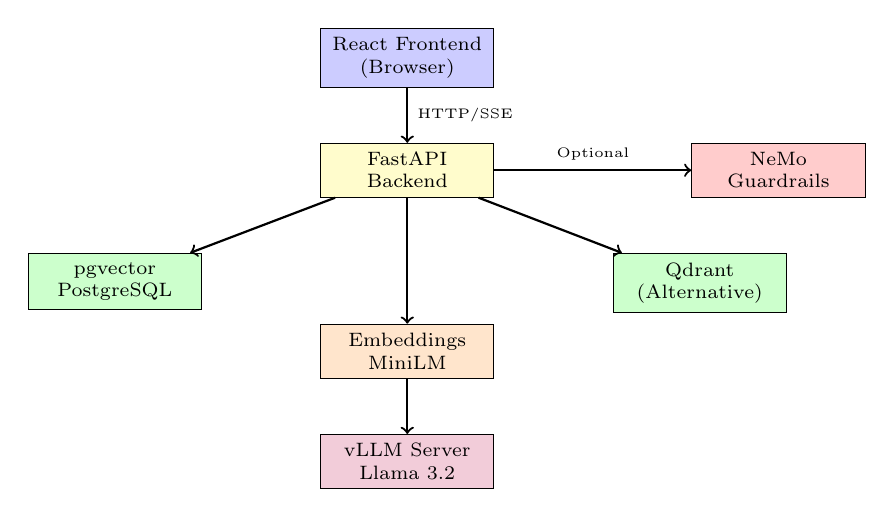
\begin{tikzpicture}[
    node distance=0.7cm,
    box/.style={rectangle, draw, minimum width=2.2cm, minimum height=0.6cm, align=center, font=\scriptsize},
    arrow/.style={->, thick}
]

% Nodes
\node[box, fill=blue!20] (browser) {React Frontend\\(Browser)};
\node[box, below=of browser, fill=yellow!20] (api) {FastAPI\\Backend};
\node[box, below left=0.7cm and 1.5cm of api, fill=green!20] (pgvector) {pgvector\\PostgreSQL};
\node[box, below right=0.7cm and 1.5cm of api, fill=green!20] (qdrant) {Qdrant\\(Alternative)};
\node[box, below=1.6cm of api, fill=orange!20] (embed) {Embeddings\\MiniLM};
\node[box, below=of embed, fill=purple!20] (vllm) {vLLM Server\\Llama 3.2};
\node[box, right=2.5cm of api, fill=red!20] (guardrails) {NeMo\\Guardrails};

% Arrows
\draw[arrow] (browser) -- node[right, font=\tiny] {HTTP/SSE} (api);
\draw[arrow] (api) -- (pgvector);
\draw[arrow] (api) -- (qdrant);
\draw[arrow] (api) -- (embed);
\draw[arrow] (embed) -- (vllm);
\draw[arrow] (api) -- node[above, font=\tiny] {Optional} (guardrails);

\end{tikzpicture}
\end{center}

\vspace{0.2cm}
\small
\textbf{Flow}: User query $\to$ Embed $\to$ Vector search $\to$ RAG context $\to$ LLM $\to$ Stream response

\end{frame}

%==============================================================================
% Slide 9: Key Features \& RAG Implementation
%==============================================================================
\begin{frame}{Key Features \& RAG Implementation}

\begin{columns}
\column{0.5\textwidth}
\textbf{User-Facing Features}:
\begin{itemize}
    \item Chat interface with streaming
    \item RAG toggle (enable/disable)
    \item PDF document upload
    \item Multiple chat sessions
    \item Dark/light theme support
    \item NeMo Guardrails agents
\end{itemize}

\column{0.5\textwidth}
\textbf{RAG Components}:
\begin{itemize}
    \item \textbf{Chunking}:
        \begin{itemize}
            \item Recursive (default)
            \item Fixed-size
            \item Semantic
        \end{itemize}
    \item \textbf{Chunk size}: 1000 chars
    \item \textbf{Overlap}: 200 chars (20\%)
    \item \textbf{Retrieval}: Top-k=3, cosine similarity
    \item Dataset registry
    \item Vector store migration tools
\end{itemize}
\end{columns}

\end{frame}

%==============================================================================
% Slide 10: Evaluation Metrics -- Planned for Stage 3
%==============================================================================
\begin{frame}{Evaluation Datasets \& Metrics \textcolor{red}{[Stage 3]}}

\begin{columns}
\column{0.5\textwidth}
\textbf{Evaluation Datasets}:
\begin{itemize}
    \item \textbf{Natural Questions (NQ)}
        \begin{itemize}
            \item Google queries + Wikipedia
            \item Factoid QA (PDF use case)
        \end{itemize}
    \item \textbf{MS MARCO}
        \begin{itemize}
            \item Bing queries + 8.8M passages
            \item Large-scale ranking
        \end{itemize}
\end{itemize}

\vspace{0.3cm}

\textbf{Current Testing}:
\begin{itemize}
    \item Qualitative evaluation
    \item Manual testing
\end{itemize}

\column{0.5\textwidth}
\textbf{Retrieval Metrics}:
\begin{itemize}
    \item \textbf{MRR@10}: Position of first relevant result
    \item \textbf{Recall@20}: \% of relevant docs found
    \item \textbf{nDCG@10}: Ranking quality (best on top)
\end{itemize}

\vspace{0.3cm}

\textbf{Generation Metrics}:
\begin{itemize}
    \item \textbf{BERTScore}: Semantic similarity with gold answer
    \item \textbf{Answer Relevance}: Does answer address query?
\end{itemize}

\vspace{0.3cm}

\textbf{Efficiency}:
\begin{itemize}
    \item Query latency, memory, throughput
\end{itemize}
\end{columns}

\end{frame}

%==============================================================================
% Slide 11: Challenges
%==============================================================================
\begin{frame}{Challenges -- Encountered \& Expected}

\begin{columns}
\column{0.5\textwidth}
\textbf{Stage 1 Challenges (Solved)}:
\begin{itemize}
    \item Docker orchestration complexity
    \item vLLM GPU memory optimization
    \item PostgreSQL pgvector setup
    \item Frontend-backend SSE streaming
    \item NeMo Guardrails integration
\end{itemize}

\column{0.5\textwidth}
\textbf{Future Challenges (Stage 2/3)}:
\begin{itemize}
    \item ColBERT index size management
    \item Fair comparison methodology
    \item Benchmark dataset preparation
    \item Hyperparameter tuning
    \item Evaluation automation
\end{itemize}
\end{columns}

\vspace{0.4cm}

\begin{table}
\centering
\small
\begin{tabular}{@{}lcc@{}}
\toprule
\textbf{Aspect} & \textbf{Current (pgvector)} & \textbf{Planned (ColBERT)} \\
\midrule
Accuracy & Baseline & Higher (expected) \\
Speed & Fast & Slower \\
Index Size & Moderate & Larger \\
\bottomrule
\end{tabular}
\end{table}

\end{frame}

%==============================================================================
% Slide 13: Timeline & Questions
%==============================================================================
\begin{frame}{Project Timeline \& Questions}

\textbf{Project Stages}:
\begin{enumerate}
    \item \textbf{Stage 1 -- COMPLETED (Nov 2025)}:
        \begin{itemize}
            \item Production RAG baseline application
            \item pgvector integration
            \item NeMo Guardrails implementation
            \item Full-stack deployment (React + FastAPI + vLLM)
        \end{itemize}
    \item \textbf{Stage 1.5 -- IN PROGRESS}:
        \begin{itemize}
            \item ColBERT prototype (RAGatouille)
            \item Standalone module, requires integration
        \end{itemize}
    \item \textbf{Stage 2 -- Planned}: Fully integrate ColBERT, HippoRAG and FAISS
    \item \textbf{Stage 3 -- Planned}: Benchmark evaluation (MS MARCO, NQ)
    \item \textbf{Stage 4 -- Final}: Comparative analysis \& report
\end{enumerate}

\vspace{0.2cm}

\begin{center}
\Large
\textbf{Questions?}

\vspace{0.1cm}

\normalsize
Thank you for your attention!
\end{center}

\end{frame}

\end{document}
